% Figure 1.3 (Session 1): the self-consistency loop and the two mean-field solutions.
% The image is rendered by figures/blender/s1_3_scf_loop.py; the coordinates of the labels
% come from figures/blender/out/scf_loop_anchors.tex. Compile with:
%   pdflatex scf_loop.tex ; result moves to ../classical_magnetism/scf_loop.pdf
\documentclass[11pt,tikz,border=0pt]{standalone}
\usepackage{amsmath,amssymb,graphicx}
\usepackage{xcolor}
\definecolor{coursedark}{HTML}{1B2A4A}
\definecolor{costamber}{HTML}{B8620A}
\newlength{\figw}\setlength{\figw}{16.19cm}   % the text width of the notes (letter, 2.7 cm margins), so labels print at size

\begin{document}
\begin{tikzpicture}[lbl/.style={font=\small, text=coursedark}]
  \node[anchor=south west, inner sep=0pt] at (0,0)
    {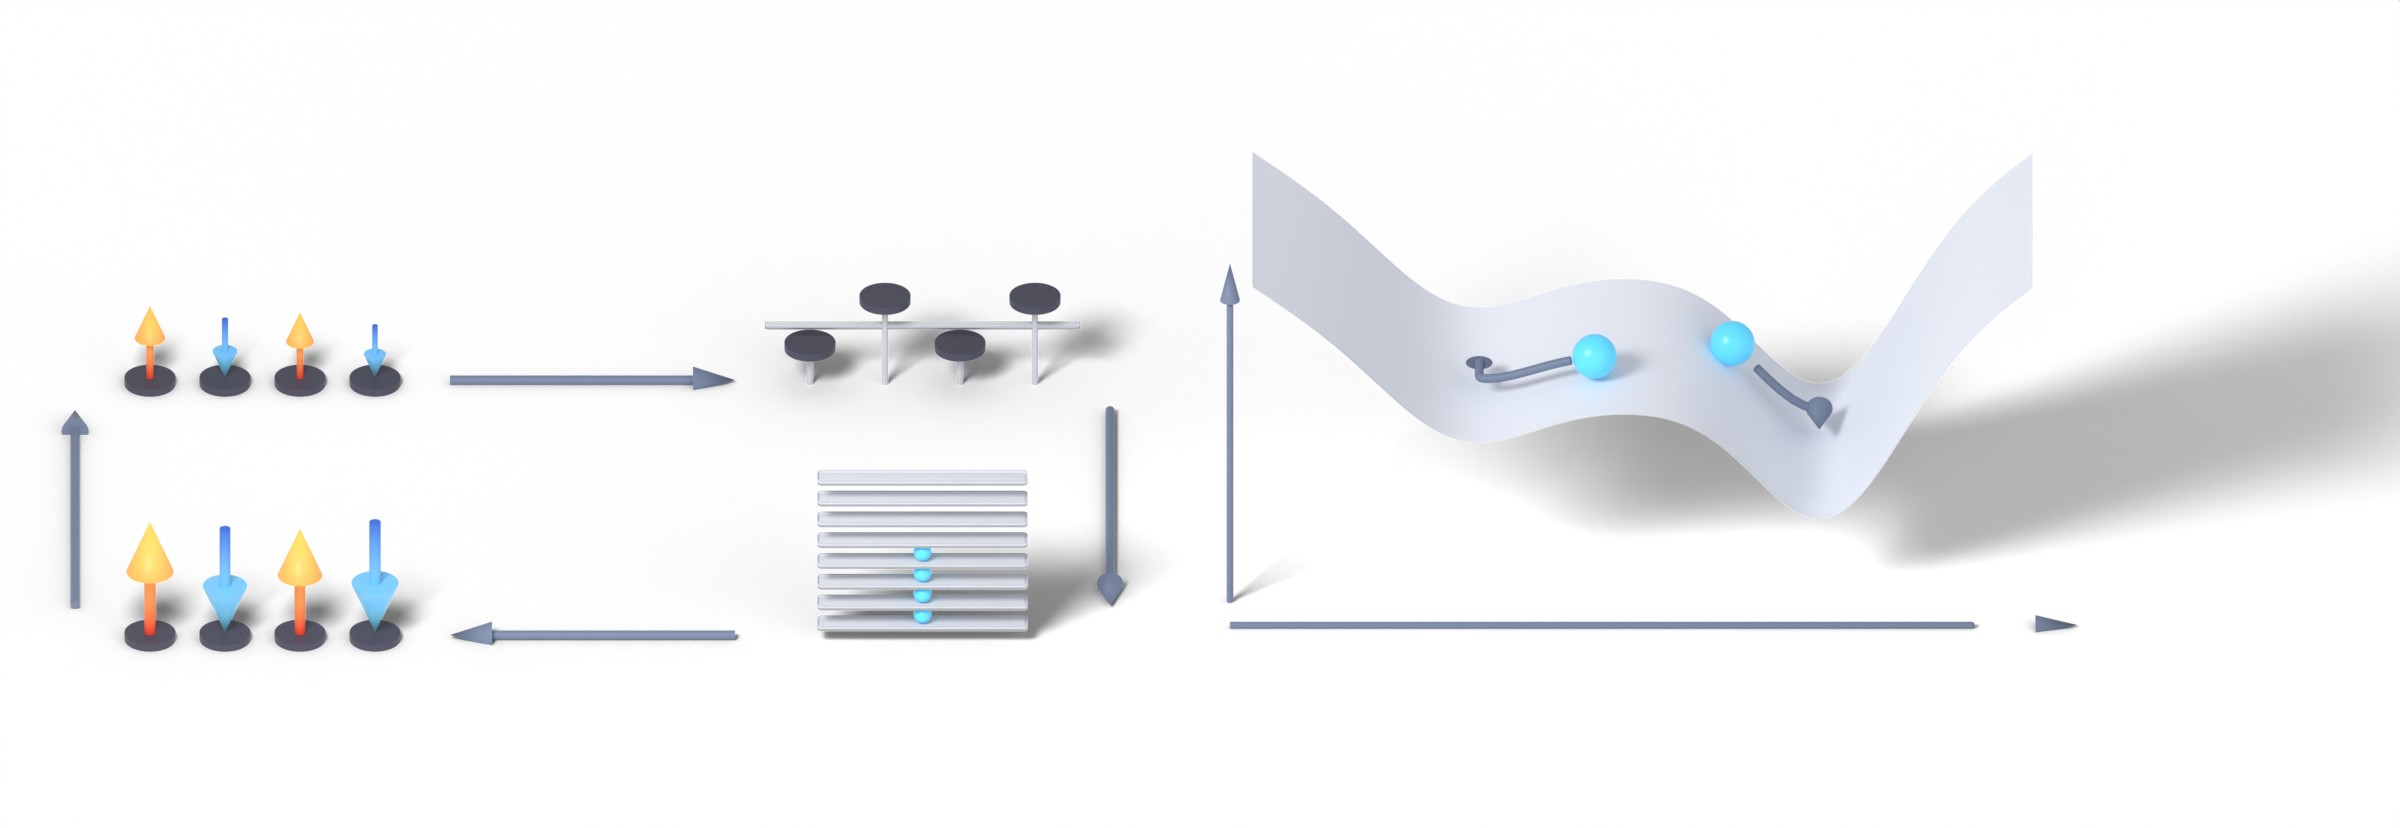
\includegraphics[width=\figw]{../blender/out/scf_loop.jpg}};
  %% written by figlib.py; x and y in units of the image width
\coordinate (st1) at (0.1094\figw,0.2419\figw);
\coordinate (st2) at (0.3844\figw,0.2310\figw);
\coordinate (st3) at (0.3844\figw,0.0647\figw);
\coordinate (st4) at (0.1094\figw,0.0647\figw);
\coordinate (mix) at (0.0250\figw,0.1319\figw);
\coordinate (N) at (0.4344\figw,0.1156\figw);
\coordinate (a) at (0.0281\figw,0.3149\figw);
\coordinate (g1) at (0.6644\figw,0.2090\figw);
\coordinate (g2) at (0.7219\figw,0.2144\figw);
\coordinate (Eax) at (0.5125\figw,0.2378\figw);
\coordinate (m) at (0.8687\figw,0.0846\figw);
\coordinate (FM) at (0.6062\figw,0.1567\figw);
\coordinate (AFM) at (0.7625\figw,0.1242\figw);
\coordinate (b) at (0.5094\figw,0.3149\figw);

  \node[lbl, font=\normalsize, anchor=west] at (a) {(a)};
  \node[lbl, font=\normalsize, anchor=west] at (b) {(b)};
  \node[lbl, anchor=south] at (st1) {1.\ guess $m_i^{(0)}$};
  \node[lbl, anchor=south] at (st2) {2.\ build $\mathcal{H}_{\mathrm{MF}}$};
  \node[lbl, anchor=north] at (st3) {3.\ fill up to $N$};
  \node[lbl, anchor=north] at (st4) {4.\ new $m_i$};
  \node[lbl, anchor=east] at (mix) {mix};
  \node[lbl, anchor=north] at (FM) {FM};
  \node[lbl, anchor=north] at (AFM) {AFM};
  \node[lbl, anchor=south] at (Eax) {$E_{\mathrm{MF}}$};
  \node[lbl, anchor=west] at (m) {$m$};
\end{tikzpicture}
\end{document}
